\fig{fv:f6:rms}{有效值由平方的平均确定，与电流代数平均不同}{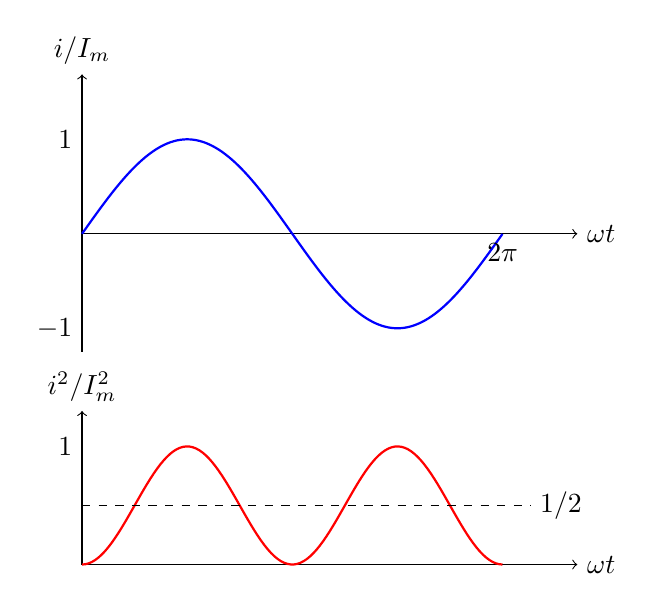
\begin{tikzpicture}[x=.85cm,y=.75cm]
\draw[->](0,0)--(7.4,0)node[right]{$\omega t$};\draw[->](0,-2)--(0,2.7)node[above]{$i/I_m$};
\draw[blue,thick,domain=0:6.283,samples=130]plot(\x,{1.6*sin(\x r)});\node[below]at(6.283,0){$2\pi$};\node[left]at(0,1.6){$1$};\node[left]at(0,-1.6){$-1$};
\begin{scope}[yshift=-4.2cm]\draw[->](0,0)--(7.4,0)node[right]{$\omega t$};\draw[->](0,0)--(0,2.6)node[above]{$i^2/I_m^2$};
\draw[red,thick,domain=0:6.283,samples=130]plot(\x,{2*sin(\x r)^2});\draw[dashed](0,1)--(6.7,1)node[right]{$1/2$};\node[left]at(0,2){$1$};\end{scope}
\end{tikzpicture}}
图\ref{fv:f6:rms}上图一个周期的有向面积为零，说明电流代数平均为零；下图平方始终非负，平均值为 $I_m^2/2$。电阻发热由 $R\int i^2\dd t$决定，与产生同样热量的直流相比，故 $I_{\rm rms}=I_m/\sqrt2$。这个系数只属于正弦波；半波整流、削顶或脉冲电流都应对其实际波形重新平方积分，不能只从峰值直接换算。
